Durante años, el estudio de las sucesiones ha sido fundamental en la teoría de 
números y en el análisis. Una de las sucesiones más relevantes es la sucesión formada
por las partes fraccionarias de los múltiplos de un número real $\alpha$,
\[
  \partfrac{\alpha}, \, \partfrac{2\alpha}, \, \partfrac{3\alpha}, \, \ldots, \, \partfrac{n\alpha}, \, \ldots
\]
donde $\partfrac{x}$ es la parte fraccionaria de $x$. 

El comportamiento de esta sucesión depende de $\alpha$. Si es racional, la 
sucesión es periódica y toma un número finito de valores. Sin embargo, cuando 
$\alpha$ es irracional, la sucesión deja de ser periódica y no se repite. 
En este caso, surge la pregunta de cómo se distribuyen los valores. 

En el siglo XIX, Kronecker demostró que si $\alpha$ es irracional, 
entonces la sucesión es densa en el intervalo $[0,1)$. Más tarde, entre 1909 y
1910, Bohl, Sierpiński y Weyl demostraron de manera independiente que esta 
sucesión no solo es densa, sino que también es equidistribuida. Este último,
Weyl, desarrolló una teoría general para el estudio de la distribución de 
sucesiones en~$[0,1)$.

En este capítulo, exploraremos los conceptos básicos para estudiar este tipo 
de problemas y los usaremos para demostrar el resultado Weyl, la equidistribución
de la sucesión $\partfrac{n\alpha}$ cuando $\alpha$ es un número irracional. 

\section{Números reales módulo 1}

\begin{definition}
    Se define la parte entera de un número $x\in \mathbb{R}$ como 
    \[
        \floor{x} = \max \{k \in \mathbb{Z}: k \leq x\}.
    \]
\end{definition} 

\begin{definition}
    Se define la parte fraccionaria de un número $x\in \mathbb{R}$ como
    \[
        \partfrac{x} = x - \floor{x}.
    \]
    Por definición, se tiene que $\partfrac{x} \in [0,1)$ para todo $x \in \mathbb{R}$.
\end{definition}

Ahora, en $\mathbb{R}$, consideramos la relación de equivalencia dada por $x \sim y$ 
si y solo si $x - y \in \mathbb{Z}$. Es decir, dos números son congruentes
módulo $\mathbb{Z}$ o módulo $1$ si difieren por un número entero. Lo indicamos con
\[
    x \equiv y \mod \mathbb{Z} \qquad \text{ o } \qquad x \equiv y \mod 1
\]

Cada clase de equivalencia tiene un representante único en el intervalo $[0,1)$ que es
justamente la parte fraccionaria $\partfrac{x}$. Podemos pensar en el conjunto cociente 
$\mathbb{R}/\mathbb{Z}$ como el intervalo $[0,1)$ al identificar sus extremos $0$ y $1$.
Este espacio se denota por $\mathbb{T}$, el toro unidimensional o la circunferencia unitaria.

A lo largo del trabajo, utilizaremos $\mathbb{T}$ para referirnos al intervalo $[0,1)$ 
con la identificación de sus extremos. 

\begin{remark}
    Las funciones en $\mathbb{T}$ son funciones $f$ $1$-periódicas en $\mathbb{R}$. Es decir,
    \[
        f(x+1) = f(x) \quad \text{ para todo } x \in \mathbb{R}.
    \]
    Debido a esta periodicidad, tenemos que $f(x) = f(\partfrac{x})$ para todo $x \in \mathbb{R}$,
    por lo que podemos considerar a $f$ como una función definida en $\mathbb{T}$.
\end{remark}

\section{Equidistribución de sucesiones}

\begin{definition}
    Sea $x=(x_n)_{n\geq1}$ una sucesión de números reales. Decimos que $(x_n)$ es
    equidistribuida módulo $1$ si para cada
    intervalo $(a,b) \subset \mathbb{T}$ con $0 < a < b < 1$ se cumple que
    \begin{align}
        \label{def:equidistribucion}
        \lim_{N\to\infty} \frac{A_N((a,b), x)}{N} = b-a
    \end{align}
    donde 
    \[
        A_N((a,b), x) = \card \left\{1\le n\le N : \partfrac{x_n} \in (a,b)\right\}
    \]
\end{definition}

\begin{remark}
    \label{obs:equidistribucion}
    Si consideramos la función característica $\mathbf{1}_{(a,b)}$ en $\mathbb{T}$, entonces la
    condición de equidistribución se puede reescribir como
    \[
        \lim_{N\to\infty} \frac{1}{N} \sum_{n=1}^N \mathbf{1}_{(a,b)}(x_n) =
        \int_0^1 \mathbf{1}_{(a,b)}(x)\ dx = 
        b-a
    \]
\end{remark}

Podemos pensar que, cuando una sucesión es equidistribuida módulo $1$, sus términos se distribuyen
de manera equitativa a lo largo de $\mathbb{T}$. En particular, la proporción de términos que 
pertenecen a un subintervalo es igual a la longitud de dicho intervalo.

La siguiente proposición permite utilizar cualquier tipo de intervalo para
verificar la equidistribución de una sucesión.

\begin{proposition}
    \label{prop:equivalentes}
    Sea $x=(x_n)_{n\geq1}$ una sucesión de números reales.
    Las siguientes afirmaciones son equivalentes:
    \begin{enumerate}
        \item $(x_n)$ es equidistribuida módulo $1$.

        \item La igualdad (\ref{def:equidistribucion}) se cumple
        para todo intervalo $(a,b)$ con $0 \leq a < b \leq 1$.

        \item La igualdad (\ref{def:equidistribucion}) se cumple
        para todo intervalo $[a,b], \,[a,b), \,(a,b]$ con $0 \leq a < b \leq 1$.

        \item La igualdad (\ref{def:equidistribucion}) se cumple
        para todo intervalo $[0,b)$ con $0 \leq b \leq 1$.

        \item La igualdad (\ref{def:equidistribucion}) se cumple
        para todo intervalo $(a,1)$ con $0 \leq a \leq 1$.

        \item La igualdad (\ref{def:equidistribucion}) se cumple
        para todo intervalo $(a,b)$ con $a,b\in D$, donde $D \subseteq \mathbb{T}$ es un conjunto denso.
    \end{enumerate}
\end{proposition}

\begin{proof}
    La demostración es técnica y se incluye en el apéndice \ref{def:equivalentes}.
\end{proof}

\begin{proposition}
    \label{prop:quitar_terminos}
    Sea $x=(x_n)_{n\geq1}$ una sucesión equidistribuida módulo $1$.  Si eliminamos
    un número finito de términos, la sucesión resultante sigue siendo equidistribuida módulo $1$.
\end{proposition}

\begin{proof}
    Sin pérdida de generalidad, supongamos que eliminamos los primeros $M$ términos de la sucesión 
    y sea $y=(y_n)_{n\geq1}$, definimos $y_n = x_{n+M}$ para cada $n \in \mathbb{N}$. 
    
    Sea $(a,b) \subset \mathbb{T}$,    
    \[
        A_N((a,b),y) = \card \left\{M+1 \leq n \leq N+M : \partfrac{x_n} \in (a,b)\right\}
    \]
    por lo que,
    \[
        A_N((a,b),y) = A_{N+M}((a,b),x) - A_M((a,b),x)
    \]

    Como $0 \leq A_M((a,b),x) \leq M$ y la sucesión $(x_n)$ es equidistribuida, 
    \[
        \lim_{N \to \infty} \frac{A_N((a,b),y)}{N} =
        \lim_{N \to \infty}  \left(\frac{N+M}{N} \, \frac{A_{N+M}((a,b),x)}{N+M} - \frac{A_M((a,b),x)}{N} \right) =
        b-a
    \]

    Por lo tanto, la sucesión $(y_n)$ es equidistribuida módulo $1$.
\end{proof}


\begin{proposition}
    \label{prop:secuencia_mas_const}
    Sea $x=(x_n)_{n\geq1}$ una sucesión equidistribuida módulo $1$
    y sea $\alpha \in \mathbb{R}$. Entonces la sucesión $y=(y_n)_{n\geq1}$ dada por
    $
        y_n = x_n + \alpha
    $
    también es equidistribuida módulo $1$.
\end{proposition}

\begin{proof}
    Sea $I=(a,b) \subset \mathbb{T}$ con $0 < a < b < 1$, definimos $J = I - \alpha \mod 1$.
    Para cada $n \in \mathbb{N}$, tenemos que
    \[
        \partfrac{y_n} \in I
        \iff \partfrac{x_n + \alpha} \in I
        \iff \partfrac{x_n} \in J
    \]
    luego
    \[
        A_N(I,y)=A_N(J,x)
    \]

    Como $(x_n)$ es equidistribuida módulo $1$ y la medida es invariante por traslaciones, se tiene
    \[
        \lim_{N\to\infty} \frac{A_N(I,y)}{N} =
        \lim_{N\to\infty} \frac{A_N(J,x)}{N} =
        |J|=|I|
    \]
    demostrando que $(y_n)$ es equidistribuida módulo $1$.
\end{proof}


\begin{example}
    Consideremos una sucesión de racionales $r=(r_n)_{n\geq1}$. Definimos la sucesión 
    $x=(x_n)_{n\geq1}$ por
    \[
        x_n = 
        \begin{cases} 
            r_{n/2} & \text{si $n$ es par} \\ 
            0 & \text{si $n$ es impar}
        \end{cases} 
    \]

    Entonces $(x_n)$ no es equidistribuida módulo $1$.
\end{example}

\begin{resolve}
    Consideramos $[0,b) \subset \mathbb{T}$ con $b < 1/2$. Si la sucesión fuese
    equidistribuida módulo $1$, debería cumplirse que
    \[
        \lim_{N\to\infty} \frac{A_N([0,b),x)}{N}  = b
    \]

    Sin embargo, para $N=2M$,
    \[
        A_{2M}([0,b),x) = M + R \qquad \text{donde } R = A_M([0,b),r) 
    \]
    Los índices impares de la sucesión $(x_n)$ son iguales a $0$ y contribuyen
    con $M$ términos.
    
    Por consiguiente,
    \[
        \frac{A_{2M}([0,b),x)}{2M} = 
        \frac{M+R}{2M} \geq  
        \frac{M}{2M} = 
        \frac{1}{2}
    \] 

    Debido a que $b < 1/2$, el límite anterior no puede ser igual a $b$ 
    y por tanto $(x_n)$ no es equidistribuida módulo $1$.
\end{resolve}

\begin{example}
    La sucesión $x=(x_n)_{n\geq1}$ dada por
    \[
        0, \ 
        0, \ \frac{1}{2}, \ 
        0, \ \frac{1}{3}, \ \frac{2}{3}, \ 
        0, \ \frac{1}{4}, \ \frac{2}{4}, \ \frac{3}{4}, \ 
        0, \ \frac{1}{5}, \ \frac{2}{5}, \ \frac{3}{5}, \ \frac{4}{5}, \ 
        0, \ \dots 
    \]
    es equidistribuida módulo $1$.
\end{example}

\begin{resolve}
    Para cada $k \in \mathbb{N}$, consideramos los conjuntos $A_k = \left\{\frac{i}{k} : i = 0, 1, 2, \dots, k-1 \right\}$.
    La sucesión se puede escribir como la concatenación de estos conjuntos,
    \[
        A_1, \ A_2, \ A_3, \ A_4, \ A_5, \ \dots
    \]
    Sea $(a,b)$ con $a,b \notin \mathbb{Q}$, sea $k$ fijo, estudiamos cuántos elementos de $A_k$ pertenecen al intervalo,
    \[
        P_k = 
        \card \left\{ \frac{i}{k} \in A_k : \frac{i}{k} \in (a,b) \right\} =
        \card \left\{ \frac{i}{k} \in A_k : i \in (ka,kb)\right\}
    \]
    Contando el número de enteros en el intervalo $(ka,kb)$, obtenemos que 
    \[
        P_k = \floor{kb} - \floor{ka+1} + 1 = \floor{kb} - \floor{ka}
    \]

    Tomando la sucesión hasta el conjunto $A_M$, inclusive. El número de total de términos y la cantidad
    de términos que están en el intervalo $(a,b)$ es
    \[
        T_M = \sum_{k=1}^M k = \frac{M(M+1)}{2} \qquad 
        S_M = \sum_{k=1}^M P_k = \sum_{k=1}^M \left(\floor{kb} - \floor{ka}\right)
    \]

    Veamos que, contando por conjuntos, se cumple la definición de equidistribución, es decir,
    \[
        \left|\frac{S_M}{T_M} - (b-a)\right| \longrightarrow 0 \qquad \text{cuando } M \to \infty.
    \]

    Para ello, tratamos de acotarlo usando que $\partfrac{x} \in [0,1)$ para cada $x \in \mathbb{R}$,
    \begin{align*}
        \left| \frac{S_M}{T_M} - (b-a) \right| 
        =\left| \frac{S_M - T_M(b-a)}{T_M} \right| 
        &=\frac{1}{T_M}\left| \sum_{k=1}^M \left(\floor{kb} - \floor{ka}\right) - \sum_{k=1}^M k(b-a) \right| \\ 
        &=\frac{1}{T_M}\left| \sum_{k=1}^M \left(\floor{kb} - \floor{ka} - kb + ka\right) \right| \\
        &\leq\frac{1}{T_M} \sum_{k=1}^M \left|\partfrac{ka} - \partfrac{kb}\right| 
        \leq\frac{1}{T_M} \sum_{k=1}^M 1 = \frac{M}{T_M}
    \end{align*}
    
    Por lo tanto, 
    \[
        \left| \frac{S_M}{T_M} - (b-a) \right| \leq
        \frac{M}{T_M} = \frac{2}{M+1} \longrightarrow 0 \qquad \text{cuando } M \to \infty.
    \]
    
    Esto demuestra que, al contar por conjuntos, la sucesión es equidistribuida para $N = T_M$.
    Falta~comprobar que también lo es para cualquier $N$. 

    Sea $N$ tal que $T_M \leq N \leq T_{M+1}$,
    \[
        A_N((a,b), x) = S_M + R \qquad \text{con } 0 \leq R \leq P_{M+1}
    \]
    Tenemos las siguientes desigualdades,
    \[
        S_M \leq S_M + R \leq S_{M+1} 
        \quad \text{ y } \quad
        \frac{1}{T_{M+1}} \leq \frac{1}{N} \leq \frac{1}{T_M}
    \]
    Al multiplicarlas,
    \[
        \frac{S_M}{T_{M+1}} \leq \frac{S_M + R}{N} \leq \frac{S_{M+1}}{T_M}
    \]
    
    Al tomar límites cuando $M \to \infty$, y por lo tanto $N \to \infty$, obtenemos
    \begin{align*}
        \lim_{M \to \infty} \frac{T_M}{T_{M+1}} \, \frac{S_M}{T_M} \leq
        \liminf_{N \to \infty} \frac{S_M + R}{N} &\leq
        \limsup_{N \to \infty} \frac{S_M + R}{N} \leq
        \lim_{M \to \infty} \frac{T_{M+1}}{T_M} \, \frac{S_{M+1}}{T_{M+1}}  \\
        b-a \leq
        \liminf_{N \to \infty} \frac{S_M + R}{N} &\leq
        \limsup_{N \to \infty} \frac{S_M + R}{N} \leq
        b-a
    \end{align*}
    Por lo que, el límite existe y es
    \[
        \lim_{N \to \infty} \frac{A_N((a,b), x)}{N} =
        \lim_{N \to \infty} \frac{S_M + R}{N} = 
        b-a
    \]
\end{resolve}  

\begin{example}
    Sean $(x_n)_{n\geq1},(y_n)_{n\geq1}$ dos sucesiones equidistribuidas módulo $1$.
    Entonces la sucesión
    \[
        z_n = \begin{cases}
            x_k & \text{si } n = 2k-1,\\
            y_k & \text{si } n = 2k,
        \end{cases}
    \]
    también es equidistribuida módulo $1$.
\end{example}

\begin{resolve}
    Sea un intervalo $(a,b) \subset \mathbb{T}$. Consideremos $2N$ términos de la sucesión $(z_n)$, 
    \[
        A_{2N}((a,b), z) = A_N((a,b), x) + A_N((a,b), y)
    \]
    
    Teniendo en cuenta que $(x_n)$ e $(y_n)$ son equidistribuidas módulo $1$, al dividir por $2N$
    y pasar al límite, obtenemos
    \[
        \lim_{N \to \infty} \frac{A_{2N}((a,b), z)}{2N} =
        \lim_{N \to \infty} \frac{1}{2} \left( \frac{A_N((a,b), x)}{N} + \frac{A_N((a,b), y)}{N} \right) =
        b-a
    \]
    
    Por otra parte, si tomamos $2N+1$ términos de la sucesión $(z_n)$, 
    \[
        A_{2N+1}((a,b), z) = A_{2N}((a,b), z) + \mathbf{1}_{(a,b)}(x_{N+1})
    \]

    Como $0 \leq \mathbf{1}_{(a,b)}(x_{N+1}) \leq 1$, al dividir por $2N+1$ y tomando límites,
    \[
        \lim_{N \to \infty} \frac{A_{2N+1}((a,b), z)}{2N+1} =
        \lim_{N \to \infty} \left(\frac{2N}{2N+1} \frac{A_{2N}((a,b), z)}{2N} + \frac{\mathbf{1}_{(a,b)}(x_{N+1})}{2N+1} \right) =  
        b-a
    \]

    Por lo tanto, $(z_n)$ es equidistribuida módulo $1$.  
\end{resolve}


\section{Sucesión $n\alpha$}

Como cierre a este capítulo, estudiaremos la sucesión $(n\alpha)_{n\geq1}$. 
Analizaremos su comportamiento módulo $1$ en función del $\alpha$, distinguiendo si es
racional o irracional. En particular, para el caso irracional demostraremos que es 
equidistribuida módulo $1$.

\begin{proposition}
    \label{prop:periodicidad}
    Sea $\alpha \in \mathbb{R}$.
    \begin{enumerate}
        \item Si $\alpha \in \mathbb{Q}$, entonces la sucesión $(\partfrac{n\alpha})_{n\ge1}$ es periódica
        y tiene un número finito de términos distintos.
        \item Si $\alpha \notin \mathbb{Q}$, entonces la sucesión $(\partfrac{n\alpha})_{n\ge1}$ tiene
        infinitos términos distintos.
    \end{enumerate}
\end{proposition}

\begin{proof}
    \textit{1. \quad} Sea $\alpha = p/q$ con $p, q \in \mathbb{Z}$ y $q \neq 0$. Entonces,
    \[
        \partfrac{p/q}, \,
        \partfrac{2p/q}, \,
        \ldots, \,
        \partfrac{(q-1)p/q}, \,
        \partfrac{qp/q} = \partfrac{p} = 0 
    \]
    A partir de aquí, la sucesión se repite,
    \[
        \partfrac{(q+1)p/q} = \partfrac{1 + p/q} = \partfrac{p/q}.
    \]
    \textit{2. \quad} Sea $\alpha \notin \mathbb{Q}$ y supongamos que $\partfrac{n\alpha} = \partfrac{m\alpha}$ 
    para ciertos $n, m \in \mathbb{N}$ con $n \neq m$. Tenemos que
    \begin{align*}
        \partfrac{n\alpha} = \partfrac{m\alpha}
        &\iff n\alpha - \floor{n\alpha} = m\alpha - \floor{m\alpha} \\
        &\iff (n-m)\alpha = \floor{n\alpha} - \floor{m\alpha} \in \mathbb{Z}
    \end{align*}
    lo que implicaría que $\alpha \in \mathbb{Q}$. Contradicción \#.
\end{proof}


Consideramos ahora el caso en el que $\alpha \notin \mathbb{Q}$. En esta situación, 
la sucesión $(n\alpha)_{n\geq1}$ es equidistribuida módulo $1$. Para demostrar
este resultado, utilizaremos el siguiente lema.

\begin{lemma} 
    \label{lem:lema_na}
    Sea $f \in C(\mathbb{T})$ y sea $\alpha \notin \mathbb{Q}$. Entonces, 
    \[
        \frac{1}{N} \sum_{n=1}^{N} f(n\alpha) \longrightarrow \int_0^1 f(x)\ dx
        \qquad \text{cuando } N \to \infty 
    \] 
\end{lemma}

\begin{proof}
    La prueba la vamos a dividir en 4 pasos.
    
    \textit{Paso 1. } Sea $f\equiv1$,
    \[
        \frac{1}{N} \sum_{n=1}^{N} f(n\alpha) = 1
        \quad \text{ y } \quad
        \int_0^1 f(x)\,dx = 1
    \]

    \textit{Paso 2. } Sea $f(x)=e^{2\pi i k x}$ con $k\in\mathbb{Z}$.
    
    Si $k=0$ estamos en el paso 1, por lo tanto, sea $k\neq 0$ y sea $r=e^{2\pi i k \alpha}$,
    \[
        \frac{1}{N} \sum_{n=1}^{N} e^{2\pi i k n \alpha} =     
        \frac{1}{N} \sum_{n=1}^{N} r^n = 
        \frac{1}{N} \, \frac{r-r^{N+1}}{1-r}
    \]
    como $\alpha \notin \mathbb{Q}$, entonces $k\alpha \notin \mathbb{Z}$ y $r \neq 1$, 
    luego $|1-r|>0$. Obteniendo la cota,
    \[
        \left|\frac{1}{N} \sum_{n=1}^{N} r^n\right| =
        \frac{1}{N} \left|\frac{r-r^{N+1}}{1-r}\right| \leq
        \frac{2}{N|1-r|}
    \]
    De este modo,
    \[
        \lim_{N \to \infty} \frac{1}{N} \sum_{n=1}^{N} e^{2\pi i k n \alpha} = 0 
    \]

    Por otro lado, calculando la integral,
    \[
        \int_0^1 e^{2\pi i k x}\,dx = 
        \left[ \frac{e^{2\pi i k x}}{2\pi i k} \right]_0^1 =
        \frac{e^{2\pi i k}-1}{2\pi i k} = 0
    \]
    obtenemos que se cumple el lema para las exponenciales complejas.

    \textit{Paso 3. } Sea $P \in \mathcal{P}(\mathbb{T})$ un polinomio trigonométrico, 
    $P=\sum_{k=-M}^M c_k e^{2\pi i k x}$ con $c_k \in \mathbb{C}$ y $M \in \mathbb{N}$. 
    Veamos que se cumple el lema para $P$,
    \begin{align*}
        \frac{1}{N} \sum_{n=1}^{N} P(n\alpha) 
        =\frac{1}{N} \sum_{n=1}^{N} \sum_{k=-M}^M c_k e^{2\pi i k n \alpha} 
        %&=\frac{1}{N} \sum_{k=-M}^M c_k \sum_{n=1}^{N} e^{2\pi i k n \alpha} \\
        =\sum_{k=-M}^M c_k \cdot \left( \frac{1}{N} \sum_{n=1}^{N} e^{2\pi i k n \alpha}\right)
    \end{align*}
    Por el paso 2, cada término de la suma converge a $\int_0^1 e^{2\pi i k x}\,dx$, luego
    \begin{align*}
        \lim_{N \to \infty} \sum_{k=-M}^M c_k \cdot \left( \frac{1}{N} \sum_{n=1}^{N} e^{2\pi i k n \alpha}\right)    
        &=\sum_{k=-M}^M c_k \cdot \left( \lim_{N \to \infty} \frac{1}{N} \sum_{n=1}^{N} e^{2\pi i k n \alpha}\right) \\
        &=\sum_{k=-M}^M c_k \cdot \int_0^1 e^{2\pi i k x}\,dx \\
        &= \int_0^1 \sum_{k=-M}^M c_k e^{2\pi i k x}\,dx 
        =\int_0^1 P(x)\,dx
    \end{align*}
    se cumple el lema para polinomios trigonométricos.

    \textit{Paso 4. } Sea $f\in C(\mathbb{T})$, sea $\varepsilon > 0$, por el teorema 
    de Weierstrass, \ref{ap:weierstrass}, existe un polinomio trigonométrico 
    $P$ tal que 
    \[
        \sup_{x \in \mathbb{T}} |f(x)-P(x)| \leq \varepsilon
    \]
    
    Por el paso 3, sabemos que para ese $\varepsilon > 0$, existe $N_0 \in \mathbb{N}$ tal que 
    para todo $N \geq N_0$ se cumple que 
    \[
        \left|\frac{1}{N} \sum_{n=1}^{N} P(n\alpha) - \int_0^1 P(x)\,dx\right| \leq \varepsilon
    \]
    Por lo tanto, para $N \geq N_0$,
    % No se si es mejor asi o ponerlo con A, B y C 
    \begin{align*}
        \left| \frac{1}{N} \sum_{n=1}^{N} f(n\alpha) - \int_0^1 f(x)\,dx \right|
        &\leq \frac{1}{N} \sum_{n=1}^{N} |f(n\alpha) - P(n\alpha)| \\  
        & \qquad\qquad +\left| \frac{1}{N} \sum_{n=1}^{N} P(n\alpha) - \int_0^1 P(x)\,dx \right| \\
        & \qquad\qquad\qquad\qquad +\int_0^1 |f(x) - P(x)|\,dx   \\
        &\leq 3\varepsilon
    \end{align*}
    Como $\varepsilon > 0$ es arbitrario, queda demostrado el lema.     
\end{proof}

\begin{theorem}
    \label{teo:teorema_na}
    Sea $\alpha \notin \mathbb{Q}$ entonces la sucesión $(n\alpha)_{n\ge1}$ es equidistribuida módulo $1$.
\end{theorem}

\begin{proof} La demostración se basa en la observación~\ref{obs:equidistribucion}.

    Sea $(a,b) \in \mathbb{T}$, sea $\varepsilon > 0$ y sean $f_\varepsilon^-, f_\varepsilon^+ \in C(\mathbb{T})$
    funciones tales que 
    \[
       0 \leq 
       \mathbf{1}_{(a+\varepsilon, b-\varepsilon)} \leq 
       f_\varepsilon^- \leq 
       \mathbf{1}_{(a,b)} \leq 
       f_\varepsilon^+ \leq
       \mathbf{1}_{(a-\varepsilon, b+\varepsilon)} \leq
       1
    \]

    % No se si ve muy bien puede que lo quite.
    \begin{figure}
        \centering
        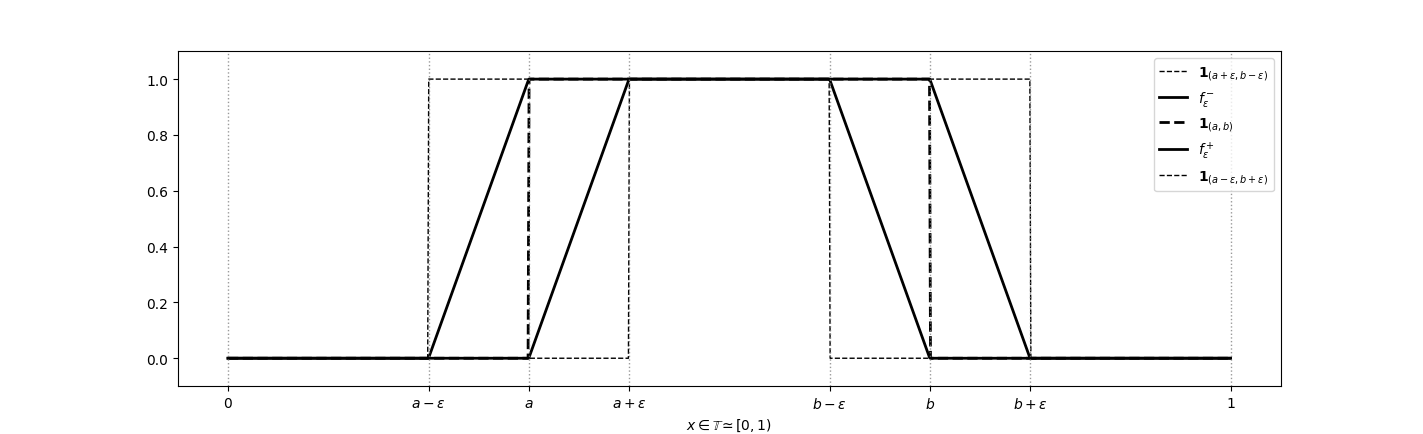
\includegraphics[scale=0.45]{pics/grafico_1_teorema_na.png}
        \caption{Gráfico de las funciones $\mathbf{1}_{(a+\varepsilon, b-\varepsilon)}$, 
        $f_\varepsilon^-$, $\mathbf{1}_{(a,b)}$, $f_\varepsilon^+$ y $\mathbf{1}_{(a-\varepsilon, b+\varepsilon)}$
        para el caso $(a,b) = (0.3, 0.7)$, $\varepsilon = 0.1$.}
    \end{figure}

    Sea $S_N = \sum_{n=1}^N \mathbf{1}_{(a,b)}(n\alpha)$, entonces,
    \[
        \frac{1}{N} \sum_{n=1}^N f_\varepsilon^-(n\alpha) \leq
        \frac{S_N}{N} \leq 
        \frac{1}{N} \sum_{n=1}^N f_\varepsilon^+(n\alpha)
    \]
    
    Por el lema anterior, se tiene que,
    \[
        b-a-2\varepsilon \leq
        \int_0^1 f_\varepsilon^-(x)\ dx \leq
        \liminf_{N \to \infty} \frac{S_N}{N} \leq
        \limsup_{N \to \infty} \frac{S_N}{N} \leq
        \int_0^1 f_\varepsilon^+(x)\ dx \leq
        b-a+2\varepsilon
    \]

    Finalmente, tomando el límite cuando $\varepsilon \to 0$ se obtiene,
    \[
        b-a \leq
        \liminf_{N \to \infty} \frac{S_N}{N} \leq
        \limsup_{N \to \infty} \frac{S_N}{N} \leq
        b-a
    \]

    Por lo tanto, el límite existe y
    \[
        \lim_{N \to \infty} \frac{1}{N} \sum_{n=1}^N \mathbf{1}_{(a,b)}(n\alpha) = b-a
    \]
\end{proof}




